\documentclass[11pt]{article}

\usepackage[margin=1in]{geometry}
\usepackage[T1]{fontenc}
\usepackage{lmodern}
\usepackage{microtype}
\usepackage{amsmath, amssymb}
\usepackage{booktabs}
\usepackage{longtable}
\usepackage{array}
\usepackage{tabularx}
\usepackage{tikz}
\usetikzlibrary{arrows.meta, positioning, shapes.geometric, calc, decorations.pathreplacing, backgrounds}
\usepackage{float}
\usepackage[hidelinks]{hyperref}
\usepackage{caption}
\usepackage{xcolor}
\usepackage{enumitem}
\usepackage[round]{natbib}

\setlength{\parskip}{0.5em}
\setlength{\parindent}{0pt}

\newcommand{\tzero}{t_{\text{zero}}}
\newcommand{\predstart}{\text{pred\_start}}
\newcommand{\predstop}{\text{pred\_stop}}

\title{\textbf{FLAIR Task Schematic} \\[0.3em]
       Sepsis Prediction with Antibiotic-Anchored Time-Zero}
\author{FLAIR Benchmark}
\date{\today}

\begin{document}
\maketitle

\begin{abstract}
\noindent We define a new FLAIR benchmark task that predicts \emph{imminent
first qualifying intravenous antibiotic administration} as an
operational proxy for clinician recognition of sepsis. The task fixes
time-zero ($\tzero$) at the first qualifying antibiotic event, starts
predictions at the first recorded vital sign, and stops predictions
strictly before $\tzero$ to avoid the label-leakage failure mode
documented by \citet{kamran2024sepsis}. This document surveys ten prior
operationalizations of sepsis onset, motivates the FLAIR choice, and
specifies the labeling, cohort, and censoring rules with TikZ schematics.
Input feature design is out of scope.
\end{abstract}

\section{Introduction}

Sepsis prediction is the most-studied AI use case in inpatient EHR
research, yet there is no consensus on \emph{when} a model's prediction
should be considered correct~\citep{singer2016sepsis3, rhee2019sepsis}.
The choice of time-zero changes both the label and the cohort, and
\citet{kamran2024sepsis} recently showed that the Epic Sepsis Model's
AUROC drops from 0.62 to 0.47 when predictions made \emph{after} a
clinician's first sepsis-treatment order are excluded. This is the
\emph{label-leakage} problem: when the gold label is itself an
administrative event (the antibiotic order), any prediction made after
that order trivially correlates with the outcome it is supposed to
forecast.

FLAIR's existing tasks (intubation, AKI, mortality, readmission) use
clinical events that are either clearly involuntary (deterioration,
death) or that occur at a clean state transition (ICU discharge). Sepsis
is fundamentally different: the label is a clinician action. The task
therefore must (i) pick an unambiguous anchor and (ii) censor predictions
made at or after that anchor.

\textbf{We adopt the antibiotic-anchored framework}: $\tzero$ is the
first qualifying systemic IV antibiotic, and the prediction window
terminates strictly before $\tzero$. This mirrors the evaluation
protocol of \citet{kamran2024sepsis} translated into a \emph{training
label} rather than a post-hoc evaluation gate.

\section{Survey of prior time-zero definitions}
\label{sec:survey}

Table~\ref{tab:lit} summarizes ten prior definitions and what each
implies for prediction-window start, stop, and label leakage.

\renewcommand{\arraystretch}{1.15}
{\footnotesize
\begin{longtable}{p{2.8cm} p{6.4cm} p{2.6cm} p{3.0cm}}
\caption{Operational time-zero definitions across major sepsis-prediction
studies.}\label{tab:lit}\\
\toprule
Paper / model & Time-zero rule & Prediction horizon & Stop rule \\
\midrule
\endfirsthead

\multicolumn{4}{l}{\textit{(continued from previous page)}}\\
\toprule
Paper / model & Time-zero rule & Prediction horizon & Stop rule \\
\midrule
\endhead

\bottomrule
\endfoot

\citet{seymour2016assessment} Sepsis-3 (JAMA) &
$t_{\text{susp}}$ = earlier of \{IV abx, blood culture\} provided
abx$\to$cult $\le 24$h or cult$\to$abx $\le 72$h; $t_{\text{sepsis}}$ =
$t_{\text{susp}} + (\Delta\text{SOFA}\ge 2 \text{ in } (-48, +24)\text{h})$
& --- (definition paper) & --- \\

\citet{reyna2020physionet} PhysioNet/CinC 2019 &
Seymour rule $+$ IV abx sustained $\ge$72h; $t_{\text{sepsis}}$ =
earlier of $t_{\text{susp}}, t_{\text{SOFA}}$ if
$t_{\text{SOFA}} \in (-24, +12)\text{h}$ of $t_{\text{susp}}$ &
6h ahead, hourly &
onset or discharge \\

\citet{desautels2016insight} InSight &
$t_{\text{susp}}$ = earliest culture or abx; SOFA window
$(-48, +24)\text{h}$ &
hourly, multi-horizon &
onset \\

\citet{shashikumar2021aise} DeepAISE &
Seymour rule; exclude sepsis in first 4h of ICU; ICU LOS 8h--20d &
$T\in\{4,6,8,12\}$h ahead &
onset / discharge \\

\citet{shashikumar2021composer} COMPOSER &
blood culture $+$ $\ge 4$d non-prophylactic IV abx, Seymour pairing &
continuous &
onset \\

Epic ESM\citep{wong2021external} &
proprietary; evaluated against Sepsis-3 &
every 20\,min throughout stay &
discharge \\

\citet{adams2022trews} TREWS &
Sepsis-3 with provider confirmation &
hourly until first abx or provider override &
provider confirms / abx \\

\textbf{\citet{kamran2024sepsis}} \textbf{(user-cited)} &
\textbf{Label} = composite of CDC ASE \citep{rhee2019sepsis} and
CMS SEP-1 \citep{cms2015sep1}. \textbf{Evaluation gate}: predictions are
restricted to time-points strictly \emph{before} the first ``treatment
indicator'' timestamp $\in$ \{antibiotics, blood culture, lactate, IV
fluids\}. \emph{No fixed $\Delta$-gate} --- the indicator timestamp
itself is the cutoff. &
ESM scores every 20 min throughout admission &
$\min$(first treatment indicator, sepsis criteria met, death, discharge) \\

\citet{rhee2019sepsis} CDC ASE &
$\ge 4$d qualifying abx within $\pm 2$d of blood culture $+$ eSOFA
organ dysfunction &
calendar-day &
--- \\

\citet{cms2015sep1} CMS SEP-1 &
2 SIRS criteria $+$ 1 organ dysfunction within 6h of one another &
--- &
--- \\
\end{longtable}
}

\paragraph{Implications for FLAIR.}
Three patterns emerge from Table~\ref{tab:lit}. First, the
Seymour-paired definition dominates the AI-sepsis literature but is
sensitive to culture order timing, which itself reflects clinician
suspicion. Second, no two studies use the same cohort entry rule:
ICU-only \citep{desautels2016insight, shashikumar2021aise} vs.
hospital-wide \citep{kamran2024sepsis, wong2021external} vs.
ED-onset~\citep{henry2022trews} produce materially different prevalence
estimates. Third, \citet{kamran2024sepsis} is the first study to
\emph{quantify} the cost of label leakage by re-evaluating an existing
deployed model under a stricter "before clinician action" rule. We
adopt their pre-treatment-indicator gate as a structural property of the
training label itself.

\section{FLAIR operational definition}
\label{sec:def}

\subsection{Anchors and windows}

Let $H_i$ denote a hospitalization with admission time
$t^{\text{adm}}_i$ and discharge or death time $t^{\text{end}}_i$.

\begin{description}[leftmargin=2em, style=nextline]

\item[Time-zero ($\tzero$).]
$\tzero^i = \min\{\,t \mid \text{med\_admin}(i,t) \in
\mathcal{A}_{\text{IV-systemic}}\,\}$ where $\mathcal{A}_{\text{IV-systemic}}$
is the curated systemic-IV-antibiotic drug list (excludes topicals,
prophylaxis single-doses, oral abx).

\item[Prediction-window start ($\predstart$).]
$\predstart_i = \min\{\,t \mid \text{vitals}(i, t) \ne \emptyset\,\}$
--- the first recorded vital sign per hospitalization. Floor at
$t^{\text{adm}}_i + 1\text{h}$ to guarantee a non-degenerate window when
vitals are taken immediately at admission.

\item[Prediction-window stop ($\predstop$).]
$\predstop_i = \min(\tzero^i,\ t^{\text{end}}_i)$.
The interval $[\predstart_i, \predstop_i)$ is closed-open;
$\tzero^i$ itself is \emph{not} a decision point.

\item[Decision-point grid.]
Hourly grid:
$D_i = \{\predstart_i + k\!\cdot\!1\text{h}\ :\ k\in\mathbb{Z}_{\ge 0},\
\predstart_i + k\!\cdot\!1\text{h} < \predstop_i\}$.

\item[Label (\texttt{label\_sepsis\_abx\_6h}).]
For $d \in D_i$:
\[
y_i(d) = \mathbb{1}\!\left[ \tzero^i \in (d,\ d + 6\text{h}\,] \right].
\]
Patients with no qualifying antibiotic ever
($\tzero^i = +\infty$) contribute all-negative rows over the entire
$[\predstart_i, t^{\text{end}}_i)$.

\end{description}

\subsection{Cohort}

Hospital-wide, mirroring \citet{kamran2024sepsis}:

\begin{itemize}[leftmargin=2em]
  \item Age at admission $\ge 18$ with valid \texttt{admission\_dttm}
        and \texttt{discharge\_dttm}.
  \item Exclude hospitalizations on psychiatric or rehabilitation
        units (Kamran 2024, Methods).
  \item Exclude $\tzero^i \le \predstart_i$ (admitted-with-treatment;
        Kamran 2024: ``patients \ldots who received treatment before the
        first measurement of vital signs'').
  \item Exclude hospitalizations with no vital-sign measurements
        (cannot anchor $\predstart$).
\end{itemize}

\subsection{Sensitivity arms (documentation only, not primary output)}

\begin{itemize}[leftmargin=2em]
  \item \textbf{ICU-only arm.} Restrict to hospitalizations with
        $\ge 1$ ICU ADT record;
        $\predstart_i = \max(\text{first\_icu\_start}_i + 1\text{h},\,
        \text{first vital})$.
  \item \textbf{Seymour-paired arm.} Require blood culture in
        $(\tzero - 72\text{h},\, \tzero + 24\text{h})$ for the
        antibiotic to qualify.
  \item \textbf{Sepsis-3 label arm.} Replace abx-as-label with
        $\Delta\text{SOFA}\ge 2$ within $\pm 48$h of $t_{\text{susp}}$
        (PhysioNet 2019 rule) for direct cross-comparison.
\end{itemize}

\section{Algorithmic flow}
\label{sec:flow}

\begin{figure}[H]
\centering
% Algorithmic flowchart for FLAIR sepsis-antibiotic task build pipeline.

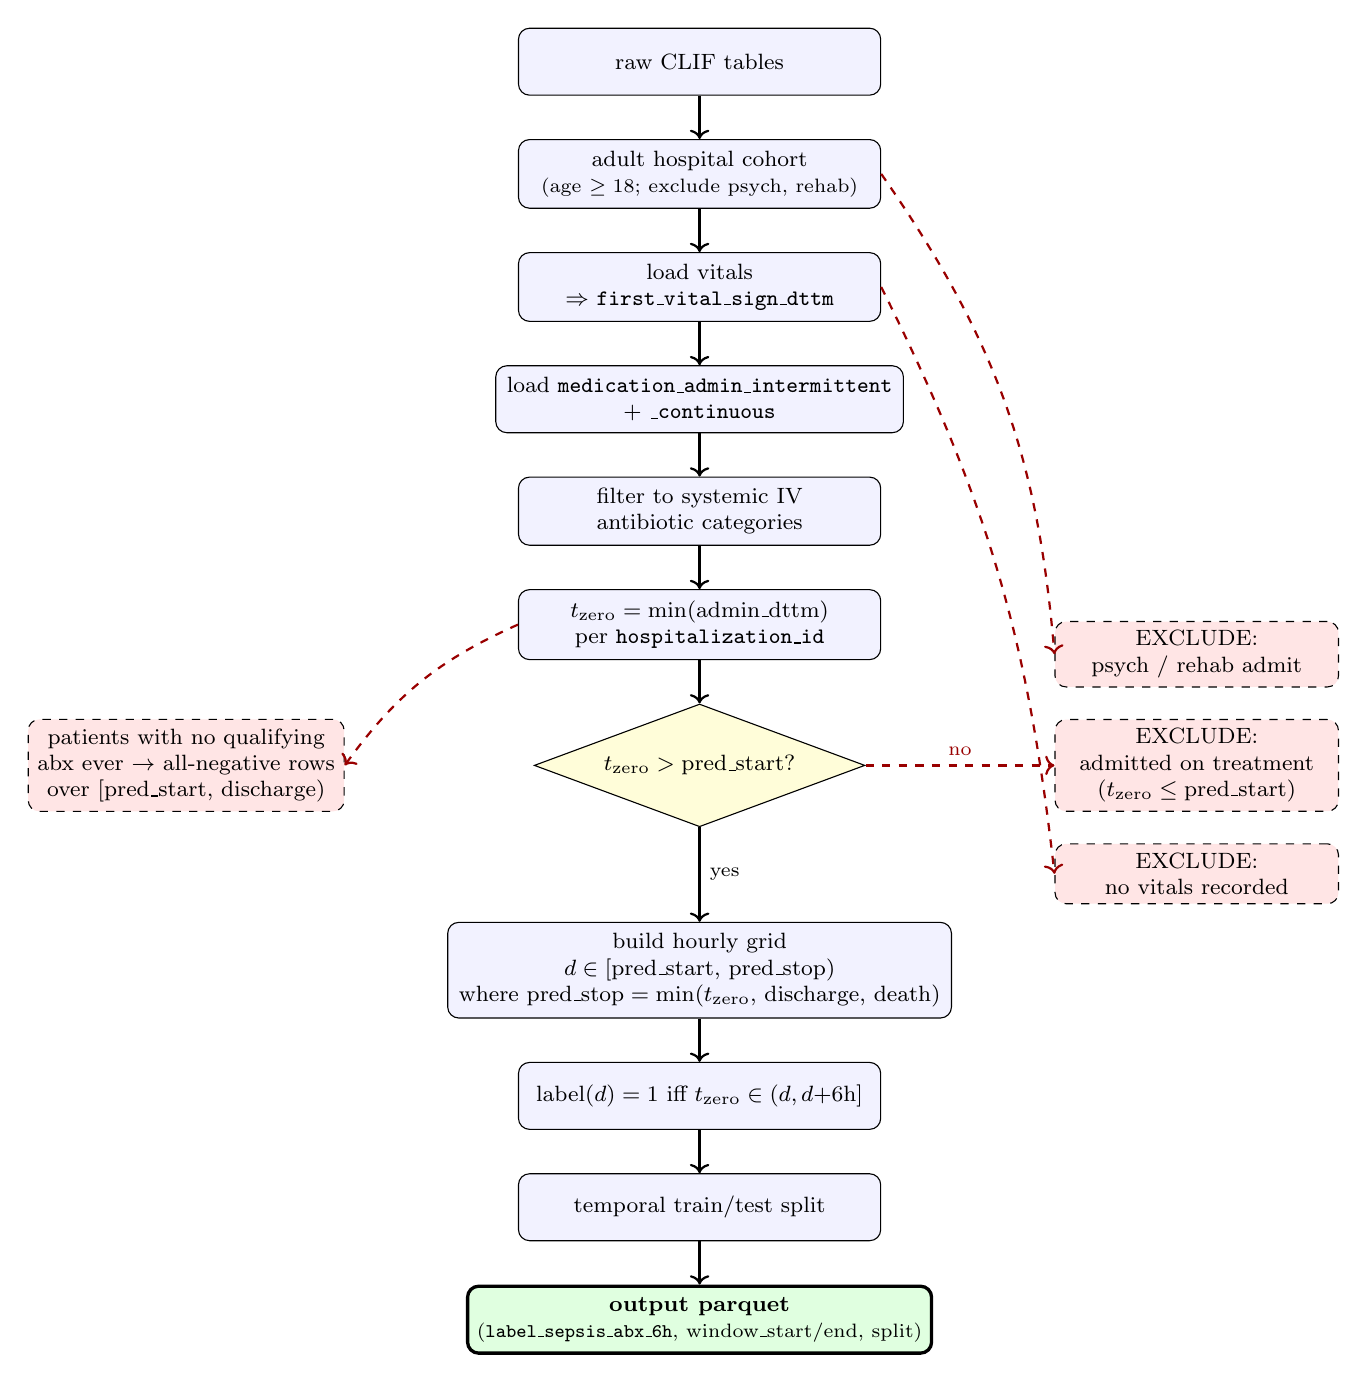
\begin{tikzpicture}[
    node distance=0.55cm and 0.7cm,
    every node/.style={font=\footnotesize, align=center},
    box/.style={draw, rounded corners, fill=blue!5,
                minimum width=4.6cm, minimum height=0.85cm, inner sep=4pt},
    dbox/.style={draw, diamond, aspect=2.2, fill=yellow!15,
                 minimum width=4.2cm, inner sep=2pt},
    excl/.style={draw, rounded corners, fill=red!10, dashed,
                 minimum width=3.6cm, minimum height=0.7cm},
    outbox/.style={draw, rounded corners, fill=green!12, very thick,
                minimum width=4.6cm, minimum height=0.85cm},
    arrow/.style={->, thick},
    sidearrow/.style={->, thick, red!60!black, dashed},
]
    % main pipeline
    \node[box] (raw) {raw CLIF tables};
    \node[box, below=of raw] (cohort)
        {adult hospital cohort\\\scriptsize(age $\geq 18$; exclude psych, rehab)};
    \node[box, below=of cohort] (vital)
        {load vitals\\$\Rightarrow$ \texttt{first\_vital\_sign\_dttm}};
    \node[box, below=of vital] (med)
        {load \texttt{medication\_admin\_intermittent}\\+ \texttt{\_continuous}};
    \node[box, below=of med] (abxf)
        {filter to systemic IV\\antibiotic categories};
    \node[box, below=of abxf] (tzero)
        {$t_{\text{zero}} = \min(\text{admin\_dttm})$\\per \texttt{hospitalization\_id}};

    \node[dbox, below=of tzero] (decide)
        {$t_{\text{zero}} > \text{pred\_start}$?};

    \node[box, below=1.2cm of decide] (grid)
        {build hourly grid\\$d \in [\text{pred\_start},\, \text{pred\_stop})$\\
         where $\text{pred\_stop} = \min(t_{\text{zero}},\, \text{discharge},\, \text{death})$};
    \node[box, below=of grid] (label)
        {label$(d) = 1$ iff $t_{\text{zero}} \in (d, d{+}6\text{h}]$};
    \node[box, below=of label] (split)
        {temporal train/test split};
    \node[outbox, below=of split] (parquet)
        {\textbf{output parquet}\\\scriptsize{(\texttt{label\_sepsis\_abx\_6h}, window\_start/end, split)}};

    % exclusions on the side
    \node[excl, right=2.4cm of decide] (exclL)
        {EXCLUDE:\\admitted on treatment\\($t_{\text{zero}} \le \text{pred\_start}$)};
    \node[excl, below=0.4cm of exclL] (exclN)
        {EXCLUDE:\\no vitals recorded};
    \node[excl, above=0.4cm of exclL] (exclP)
        {EXCLUDE:\\psych / rehab admit};
    \node[excl, left=2.4cm of decide] (negs)
        {patients with no qualifying\\abx ever $\to$ all-negative rows\\over $[\text{pred\_start},\,\text{discharge})$};

    % main arrows
    \draw[arrow] (raw) -- (cohort);
    \draw[arrow] (cohort) -- (vital);
    \draw[arrow] (vital) -- (med);
    \draw[arrow] (med) -- (abxf);
    \draw[arrow] (abxf) -- (tzero);
    \draw[arrow] (tzero) -- (decide);
    \draw[arrow] (decide) -- node[right, font=\scriptsize]{yes} (grid);
    \draw[arrow] (grid) -- (label);
    \draw[arrow] (label) -- (split);
    \draw[arrow] (split) -- (parquet);

    % exclusion arrows
    \draw[sidearrow] (decide) -- node[above, font=\scriptsize]{no} (exclL);
    \draw[sidearrow] (cohort.east) to[bend left=15] (exclP.west);
    \draw[sidearrow] (vital.east) to[bend left=10] (exclN.west);
    \draw[sidearrow] (tzero.west) to[bend right=15] (negs.east);

\end{tikzpicture}

\caption{Build pipeline. Solid arrows: main flow. Dashed red arrows:
exclusions. The diamond enforces the label-leakage gate: any
hospitalization whose qualifying antibiotic precedes its first vital
sign is dropped, since by Kamran et al.'s argument no decision point
in that stay can produce a recognition-free prediction.}
\label{fig:flow}
\end{figure}

Step-by-step prose:

\begin{enumerate}[leftmargin=2em]
  \item Load CLIF tables: \texttt{hospitalization}, \texttt{patient},
        \texttt{adt}, \texttt{vitals}, and both
        \texttt{medication\_admin\_intermittent} /
        \texttt{medication\_admin\_continuous}.
  \item Apply hospital-wide cohort filters: age, psych/rehab exclusion.
  \item Compute $\predstart_i$ from \texttt{vitals.recorded\_dttm}.
  \item Filter \texttt{medication\_admin\_*} to
        $\mathcal{A}_{\text{IV-systemic}}$; compute
        $\tzero^i = \min(\text{admin\_dttm})$ per
        \texttt{hospitalization\_id}.
  \item Apply the leakage gate: drop $\tzero^i \le \predstart_i$.
  \item Explode the hourly decision-point grid
        $[\predstart_i, \predstop_i)$ per hospitalization
        (\verb|pl.datetime_ranges|, closed-open).
  \item Assign $y_i(d)$ per the label rule.
  \item Assign \texttt{window\_start} $= d - 24\text{h}$,
        \texttt{window\_end} $= d$ (lookback window, fixed 24h to
        match the FLAIR convention).
  \item Apply temporal train/test split per
        \texttt{flair\_benchmark.\_split.assign\_split}.
  \item Select \texttt{OUTPUT\_COLS} and persist as parquet.
\end{enumerate}

\section{Timeline diagram}
\label{sec:timeline}

\begin{figure}[H]
\centering
% Timeline diagram for FLAIR sepsis-antibiotic task.
% Horizontal axis = hospitalization time (admission -> discharge).
% Markers: pred_start (first vital), t_zero (first qualifying IV abx),
% rolling 24h lookback, exclusion zone after t_zero.

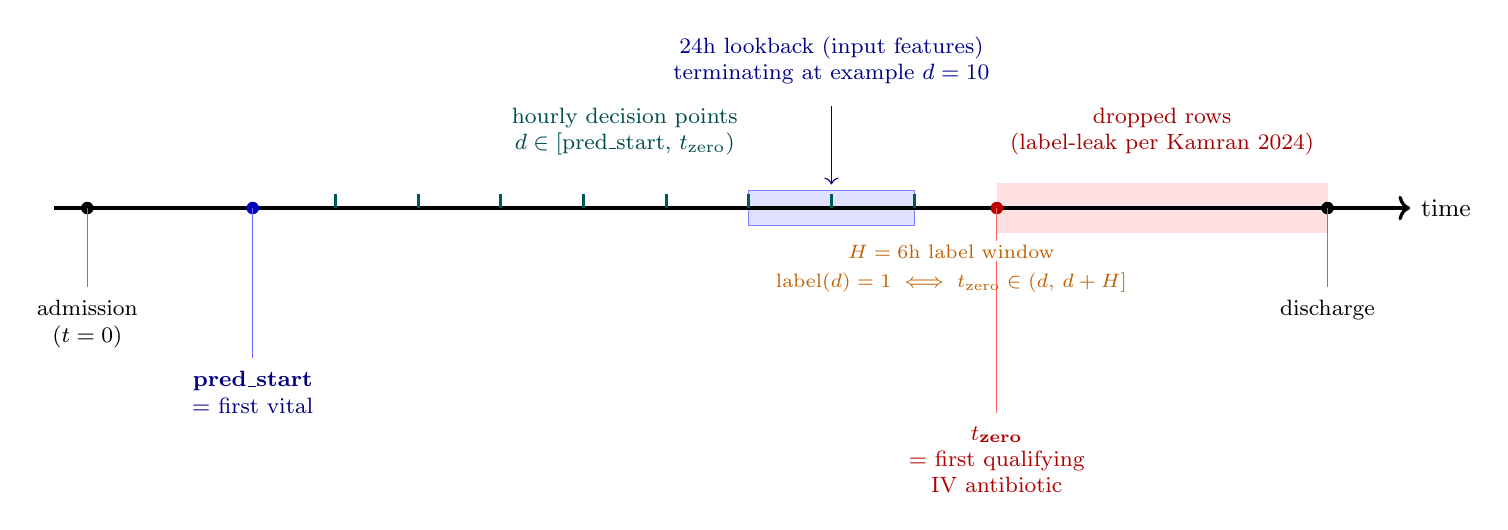
\begin{tikzpicture}[
    x=1.05cm,
    y=1cm,
    every node/.style={font=\small},
    dot/.style={circle, fill=black, inner sep=1.6pt},
    above_lbl/.style={align=center, anchor=south, font=\footnotesize},
    below_lbl/.style={align=center, anchor=north, font=\footnotesize},
    zone/.style={fill=red!12, draw=none},
    look/.style={fill=blue!12, draw=blue!50},
    decision/.style={draw=teal!70!black, line width=1.1pt},
]

    % --- exclusion zone (post-antibiotic) ---
    \fill[zone] (11,-0.32) rectangle (15,0.32);

    % --- 24h rolling lookback box at example decision point d=10 ---
    \fill[look] (8,-0.22) rectangle (10,0.22);

    % --- main time axis ---
    \draw[->, very thick] (-0.4,0) -- (16,0) node[right] {time};

    % --- key anchors with vertical offset labels to avoid collisions ---
    % admission at x=0
    \node[dot] (admit) at (0,0) {};
    \draw[gray] (0,0) -- (0,-1.0);
    \node[below_lbl] at (0,-1.05) {admission\\($t = 0$)};

    % pred_start at x=2.0
    \node[dot, fill=blue!75!black] (vital) at (2,0) {};
    \draw[blue!60] (2,0) -- (2,-1.9);
    \node[below_lbl, text=blue!50!black] at (2,-1.95)
        {\textbf{pred\_start}\\$=$ first vital};

    % t_zero at x=11
    \node[dot, fill=red!75!black] (tzero) at (11,0) {};
    \draw[red!60] (11,0) -- (11,-2.6);
    \node[below_lbl, text=red!70!black] at (11,-2.65)
        {\textbf{$t_{\text{zero}}$}\\$=$ first qualifying\\IV antibiotic};

    % discharge at x=15
    \node[dot] (disch) at (15,0) {};
    \draw[gray] (15,0) -- (15,-1.0);
    \node[below_lbl] at (15,-1.05) {discharge};

    % --- decision-point grid (hourly, schematic) between pred_start and t_zero ---
    \foreach \x in {3,4,5,6,7,8,9,10} {
        \draw[decision] (\x,0) -- (\x,0.18);
    }

    % --- TOP labels (staggered vertical heights) ---
    \node[above_lbl, text=teal!60!black] at (6.5, 0.55)
        {hourly decision points\\$d \in [\text{pred\_start},\, t_{\text{zero}})$};

    \node[above_lbl, text=blue!55!black] at (9, 1.45)
        {24h lookback (input features)\\terminating at example $d=10$};
    \draw[blue!55!black, ->, thin] (9,1.3) -- (9, 0.3);

    \node[above_lbl, text=red!65!black] at (13, 0.55)
        {dropped rows\\(label-leak per Kamran 2024)};

    % --- bottom annotation: label window for example d ---
    \draw[<->, thick, orange!75!black]
        (10, -0.55) -- node[fill=white, inner sep=1.2pt, font=\scriptsize]
        {$H = 6$h label window} (10.9, -0.55);
    \node[font=\scriptsize, orange!75!black, anchor=north]
        at (10.45, -0.7)
        {$\text{label}(d)=1 \iff t_{\text{zero}} \in (d,\, d+H]$};

\end{tikzpicture}

\caption{Hospitalization timeline. The blue ``lookback'' bar shows the
24h rolling feature window terminating at one example decision point.
The red ``dropped rows'' zone covers $[\tzero, \text{discharge})$ ---
any prediction made at or after the antibiotic order is removed from
training and evaluation, eliminating the label-leakage channel
identified by \citet{kamran2024sepsis}.}
\label{fig:timeline}
\end{figure}

\section{Design choices and rationale}
\label{sec:rationale}

\paragraph{Why antibiotic-as-anchor (not SOFA $\Delta\!\ge\!2$).}
The clinical workflow this task targets is the moment a clinician
decides to treat for suspected infection. SOFA-anchored labels
\citep{singer2016sepsis3, reyna2020physionet} describe physiology, not
action: a model that predicts SOFA deterioration may be operationally
useless if the deterioration is recognized faster than the model's lead
time. Antibiotic order is the action we want to bring forward.

\paragraph{Why strictly $\predstop = \tzero$ with no $\Delta$-gate.}
\citet{kamran2024sepsis} do not introduce a fixed buffer; they restrict
analysis to ``predictions occurring before sepsis criteria were met and
before the first indicator of treatment.'' Adding a buffer is an
additional design choice and is documented in Table~\ref{tab:lit} for
methods that adopt one. FLAIR follows the parsimonious Kamran rule: the
order timestamp itself is the cutoff.

\paragraph{Why hospital-wide (not ICU-only).}
Hospital-wide matches \citet{kamran2024sepsis}'s cohort and captures
the operationally important ward-onset sepsis cases, where prediction
lead time has the most clinical value. The ICU-only variant is
preserved as a sensitivity arm for comparability with
\citet{shashikumar2021aise} and \citet{desautels2016insight}.

\paragraph{Why hourly grid.}
Matches the FLAIR convention (task5 AKI-24h uses the same hourly grid) and
the PhysioNet/CinC 2019 standard. ESM's native 20-minute cadence
\citep{wong2021external, kamran2024sepsis} is finer than necessary for
benchmarking and would inflate row counts $\sim$3$\times$ without
adding label resolution.

\paragraph{Prevalence implications.}
Hospital-wide hourly grids produce highly imbalanced labels: a 7-day
stay with one antibiotic event produces $\le 6$ positive rows out of
$\sim$160. Reporting AUPRC alongside AUROC is mandatory, per the
\texttt{META.evaluation\_metrics} convention.

\paragraph{Drug list.}
The systemic-IV-antibiotic curation is the largest open dependency
and is deferred to a follow-up round. CLIF's \texttt{med\_category}
mapping must be extended with an
\texttt{antibiotic\_systemic\_iv} class. The list should follow
\citet{rhee2019sepsis}'s ``qualifying antimicrobial therapy''
definition (CDC ASE Appendix).

\section{Out of scope}

\begin{itemize}[leftmargin=2em]
  \item Implementation of
        \texttt{flair\_benchmark/tasks/task4\_sepsis\_abx\_6h.py}.
  \item Curated antibiotic drug list and \texttt{med\_category}
        mapping.
  \item Choice of input features and feature engineering.
  \item Sensitivity-arm output schemas.
\end{itemize}

\bibliographystyle{plainnat}
\bibliography{references}

\end{document}
